% Template for ICIP-2009 paper; to be used with:
%          spconf.sty  - ICASSP/ICIP LaTeX style file, and
%          IEEEbib.bst - IEEE bibliography style file.
% --------------------------------------------------------------------------
\documentclass{article}
\usepackage{spconf,amsmath,epsfig,subfigure}

% Example definitions.
% --------------------
\def\x{{\mathbf x}}
\def\L{{\cal L}}

% Title.
% ------
\title{BETTER COMPUTER VISION UNDER VIDEO COMPRESSION, 
AN EXAMPLE USING MEAN SHIFT TRACKING
}
%
% Single address.
% ---------------
\name{Salman Aslam, Aaron Bobick, Christopher Barnes, Osman Sezer}
\address{Georgia Institute of Technology}
%
% For example:
% ------------
%\address{School\\
%	Department\\
%	Address}
%
% Two addresses (uncomment and modify for two-address case).
% ----------------------------------------------------------
%\twoauthors
%  {Salman Aslam, Christopher Barnes, Osman Sezer}
%	{School of Electrical and Computer Engineering\\
%	Georgia Institute of Technology\\
%	Atlanta, USA}
%  {Aaron Bobick}
%	{College of Computing\\
%	Georgia Institute of Technology\\
%	Atlanta USA}
\begin{document}
\ninept

\maketitle
%
\begin{abstract}
In this paper, our goal is to understand what needs to be done to enable computer vision algorithms running on uncompressed image sequences to run as well on image sequences that have undergone compression and then decompression.    The central conflict of context based computer vision algorithms versus the structured block based approach of today's codecs means that more has to be done than to simply create a divide between coding foreground preferentially and giving less importance to background.  We take as example, a single computer vision algorithm, the mean shift tracker and see that its performance can be improved substantially in low bit rate scenarios, albeit some tradeoffs.  \end{abstract}
%
\begin{keywords}
Computer vision, MPEG-4, mean shift tracker, video compression
\end{keywords}

%--------------------------------------------------------------------------------------------------------------------------------------------------------------
\section{INTRODUCTION}
%--------------------------------------------------------------------------------------------------------------------------------------------------------------
Figure~\ref{fig:ProblemStatement} presents the overall framework we are interested in.  It can be summarized in three points (a) A video signal from a given source needs to be transmitted to another point over a bandwidth constrained system.  (b) Since bandwidth is limited, we would like to encode the video.  However, we limit ourselves to using standard widely available codecs, such as MPEG-4, H.264 etc. (c) Depending on the application, some form of information extracted from the original video needs to be preserved in the decoded video. 

\begin{figure}[h]
			\centering
			\includegraphics[width=.45\textwidth]{figs/ICIP2009_BlockDiagram_1}
			\caption{Overall framework.}
			\label{fig:ProblemStatement}
\end{figure}

Examples where such a situation may arise are many.  In surveillance applications, video cameras normally send back compressed video to a central server for analysis.  Although there is a rising trend in edge processing, i.e. processing at the camera itself, the need to transmit the video to a central server for human consumption and data fusion from other sensors still remains.  In satellite imaging applications, downlink video may be analyzed at ground stations for atmospheric and geological patters, disaster zone identification, vegetation analysis or structure classification.  In medical imaging, there is a rising trend in remote diagnosis and surgery.  In the latter case, it is absolutely essential that the most critical information in the video signal is preserved.  In these applications, and in hundreds of other applications where it is important to preserve some form of information in the video other than visual quality, the goal of coding video can be addressed in three ways (a) design a video codec tailored for each application that efficiently concentrates bits where they matter most.  The disadvantages in terms of cost, maintainability, upgradeability and cross operability are obvious (b) provide a general framework for transmitting both video and information extracted from the video in a coherent and integrated manner.  This approach was adopted by MPEG in 1993 and resulted in MPEG-4.  However, in practice, just the video coding standard was adopted and other scene construction and description features did not gain much acceptance.  Perhaps too much was attempted with too many applications in mind.  The result was a huge standard difficult to understand and implement.  In the end, just the video coding part got some acceptance.  As a matter of fact, even within the video standard, the concept of object coding provided by the Main, Core and other advanced profiles has not been widely used.  Ironically, the video coding part is being replaced by H.264 which does not include the option of object coding (c) the third and final approach is to use existing rectangular based coding standards and modify the video signal so that it is more robust to changes induced by the video compression process.  This mapping $g(I)$, where $I$ is the input signal is shown in Figure~\ref{fig:SolutionThroughSigProc}.  

\begin{figure}[h]
			\centering
			\includegraphics[width=.45\textwidth]{figs/ICIP2009_BlockDiagram_2_sigproc}
			\caption{Modified framework.}
			\label{fig:SolutionThroughSigProc}
\end{figure}

The mapping will vary from application to application.  Moreover, it can be designed in a manner that an inverse mapping is required to make the picture presentable for human consumption.  Or it may be constrained to be look like the original image so that the decoded signal remains strictly decoder compliant.  We would like to take the latter approach.  More formally, this problem can be cast as a calculus of variations problem where we seek to minimize the functional $J(g)$

\begin{equation}
\label{eq:CalcOfVarFormulation}
J(g)=\int\int_D \left\|f(I) - f(\hat{g}(I)) \right\|  +  \left\|p(I) - p(\hat{g}(I)) \right\| dxdy
\end{equation}

$\hat{g}(I)$ can be written as $C^{-1}(C(g(I(x,y)))$ where $C(x,y)$ is

\begin{equation}
\label{eq:DCT}
C(x,y) = \sum_{x_0}\sum_{y_0}T(Q(D(I)))\delta(x-kx_0, y-ky_0)
\end{equation}

where $I(x,y)$ is the original image.  $D(x,y)$ is the DCT transform of a $k$x$k$ block of image data or motion compensated residuals.  Without loss of generality in our particular setup, we use I frames and therefore the DCT transform is for $k$x$k$ blocks of image data.  The value of $k$ is normally 8.  $Q(x,y)$ is a quantization function and can depend on quantization matrices and the quantization parameter $Qp$. $T(x,y)$  is a thresholding function.  We omit the lossless parts of the compression system, such as Huffman Coding, Arithmetic Coding etc, since they do not result in distortions in our setup.  There is an additional element of numerical precision errors, particularly in the DCT setup that we choose to ignore for simplicity.  $f(x,y)$ in Equation~\ref{eq:CalcOfVarFormulation} is the particular computer vision algorithm that we're interested in, and whose performance we would like to retain, or even improve when it is run on a decoded signal.

Equation~\ref{eq:CalcOfVarFormulation} then says that over the space of all transformations that can be applied to the input image $I(x,y)$, we would like to find the transformation that minimizes the distance between the output of a computer vision algorithm $f(x,y)$ running on the original image and running on the decompressed image, and that also minimizes some similarity measure $p(x,y)$ of the image itself.  

It is clear that Equation~\ref{eq:CalcOfVarFormulation} is not differentiable, particularly due to the discontinuities on the $k$x$k$ block boundaries of DCT encoded data and the thresholding function that generates further discontinuities.  However, even if numerical schemes are resorted to, the Euler Lagrange approach of the variational problem is a necessary but not sufficient condition for global optimality.  In such cases, one can resort to finding a transform $g(x,y)$ either experimentally through Monte Carlo simulations, or using prior knowledge of the nature of the computer vision algorithm we are interested in.  We use the latter approach.  

The output of the computer vision algorithm could be a scalar, vector, matrix or any N-dimensional signal.  We will use the term feature space for it.  In general, the feature space will be distorted by the compression system since the MPEG-x and H.26x codecs have been designed to discard high frequency content.  A feature space that relies on high frequency content, such as edge and corner finding will undergo more distortion.  


%--------------------------------------------------------------------------------------------------------------------------------------------------------------
\section{EXPERIMENTS}
%--------------------------------------------------------------------------------------------------------------------------------------------------------------

In this setup, the computer vision algorithm that we choose to experiment with is the well-known Mean Shift Tracker as developed and explained in \cite{2003_JNL_TRKkernel_Comaniciu}, \cite{1998_JNL_FaceObjectTracking_Bradski}, \cite{2008_BOOK_OpenCV_Bradski}.  The goal of the mean shift algorithm is to find the peak of a distribution over time.  In our case, we use it to find the peak of the color distribution of the object we are interested in.  An initial reference hue histogram of the object we would like to track is created.  We assume that this initialization is carried out by some other process, or could be done manually.  In the case of static cameras, a background modeling algorithm such as the Multi Gaussian algorithm could be used \cite{2000_JNL_MG_Stauffer}, \cite{2005_JNL_SURVEYchangeDetection_Radke}.  However, we make no assumptions about this step, and our approach is equally valid for moving cameras.  After creating the initial histogram, subsequent images are backprojected on this histogram to create a likelihood function.  A window placed over the initial location of the target object is then placed on this backprojected window and moved to a new place as computed by the mean shift vectors, $x_c$ and $y_c$.    If a rectangular kernel for the window is used \cite{1998_JNL_FaceObjectTracking_Bradski}, \cite{2008_BOOK_OpenCV_Bradski}, then the mean shift computations reduce to finding the zeroth and first order image moments,

\begin{align}
	\label{eq:MeanShiftEquations}
	M_{00}&=\sum_x\sum_yI(x,y)\notag\\
	M_{10}&=\sum_x\sum_yxI(x,y)\notag\\
	M_{01}&=\sum_x\sum_yyI(x,y)\\
	x_c&=\frac{M_{10}}{M_{00}}\notag \\
	y_c&=\frac{M_{01}}{M_{00}} \notag
\end{align}

This step is repeated until the mean shift vectors converge.  In practice, convergence takes 3 to 4 steps, but may take up to 8 to 9 steps when the algorithm is run on an MPEG-4 decoded image.  

For the image sequences, we used two standard databases, Performance Evaluation of Tracking and Surveillance 2001 (PETS2001) and PETS2007.  

In step 1 of our experiments, ground truth tracking information was obtained by running a standard open source mean shift tracker provided in the Intel OpenCV library, on PETS2001 and PETS2007 databases as shown in Figure~\ref{fig:ExperimentalSetup}.  

\begin{figure}[h]
			\centering
			\includegraphics[width=.45\textwidth]{figs/ICIP2009_ExperimentalSetup_sigProc}
			\caption{ExperimentalSetup.}
			\label{fig:ExperimentalSetup}
\end{figure}

In step 2, the mean shift tracker was run on MPEG-4 coded image sequences.  The codec used is a standard MPEG-4 Part 2 Visual codec obtained from ISO.  The reason for not using an H.264 codec was that some of our initial experiments tried to use object based functionality of this codec, which is not provided in H.264.  The tracking performance of the mean shift algorithm degraded on the outputs of the MPEG-4 codec, as expected.  The quality of the video was changed using the quantization parameter $Qp$.  Quantization matrices were not adjusted.  $Qp$ is stored in 5 bits and therefore takes on the values in [1,31].  From here on, this is called Tracker 1.

%PETS2001: picture
\begin{figure}
			\centering
			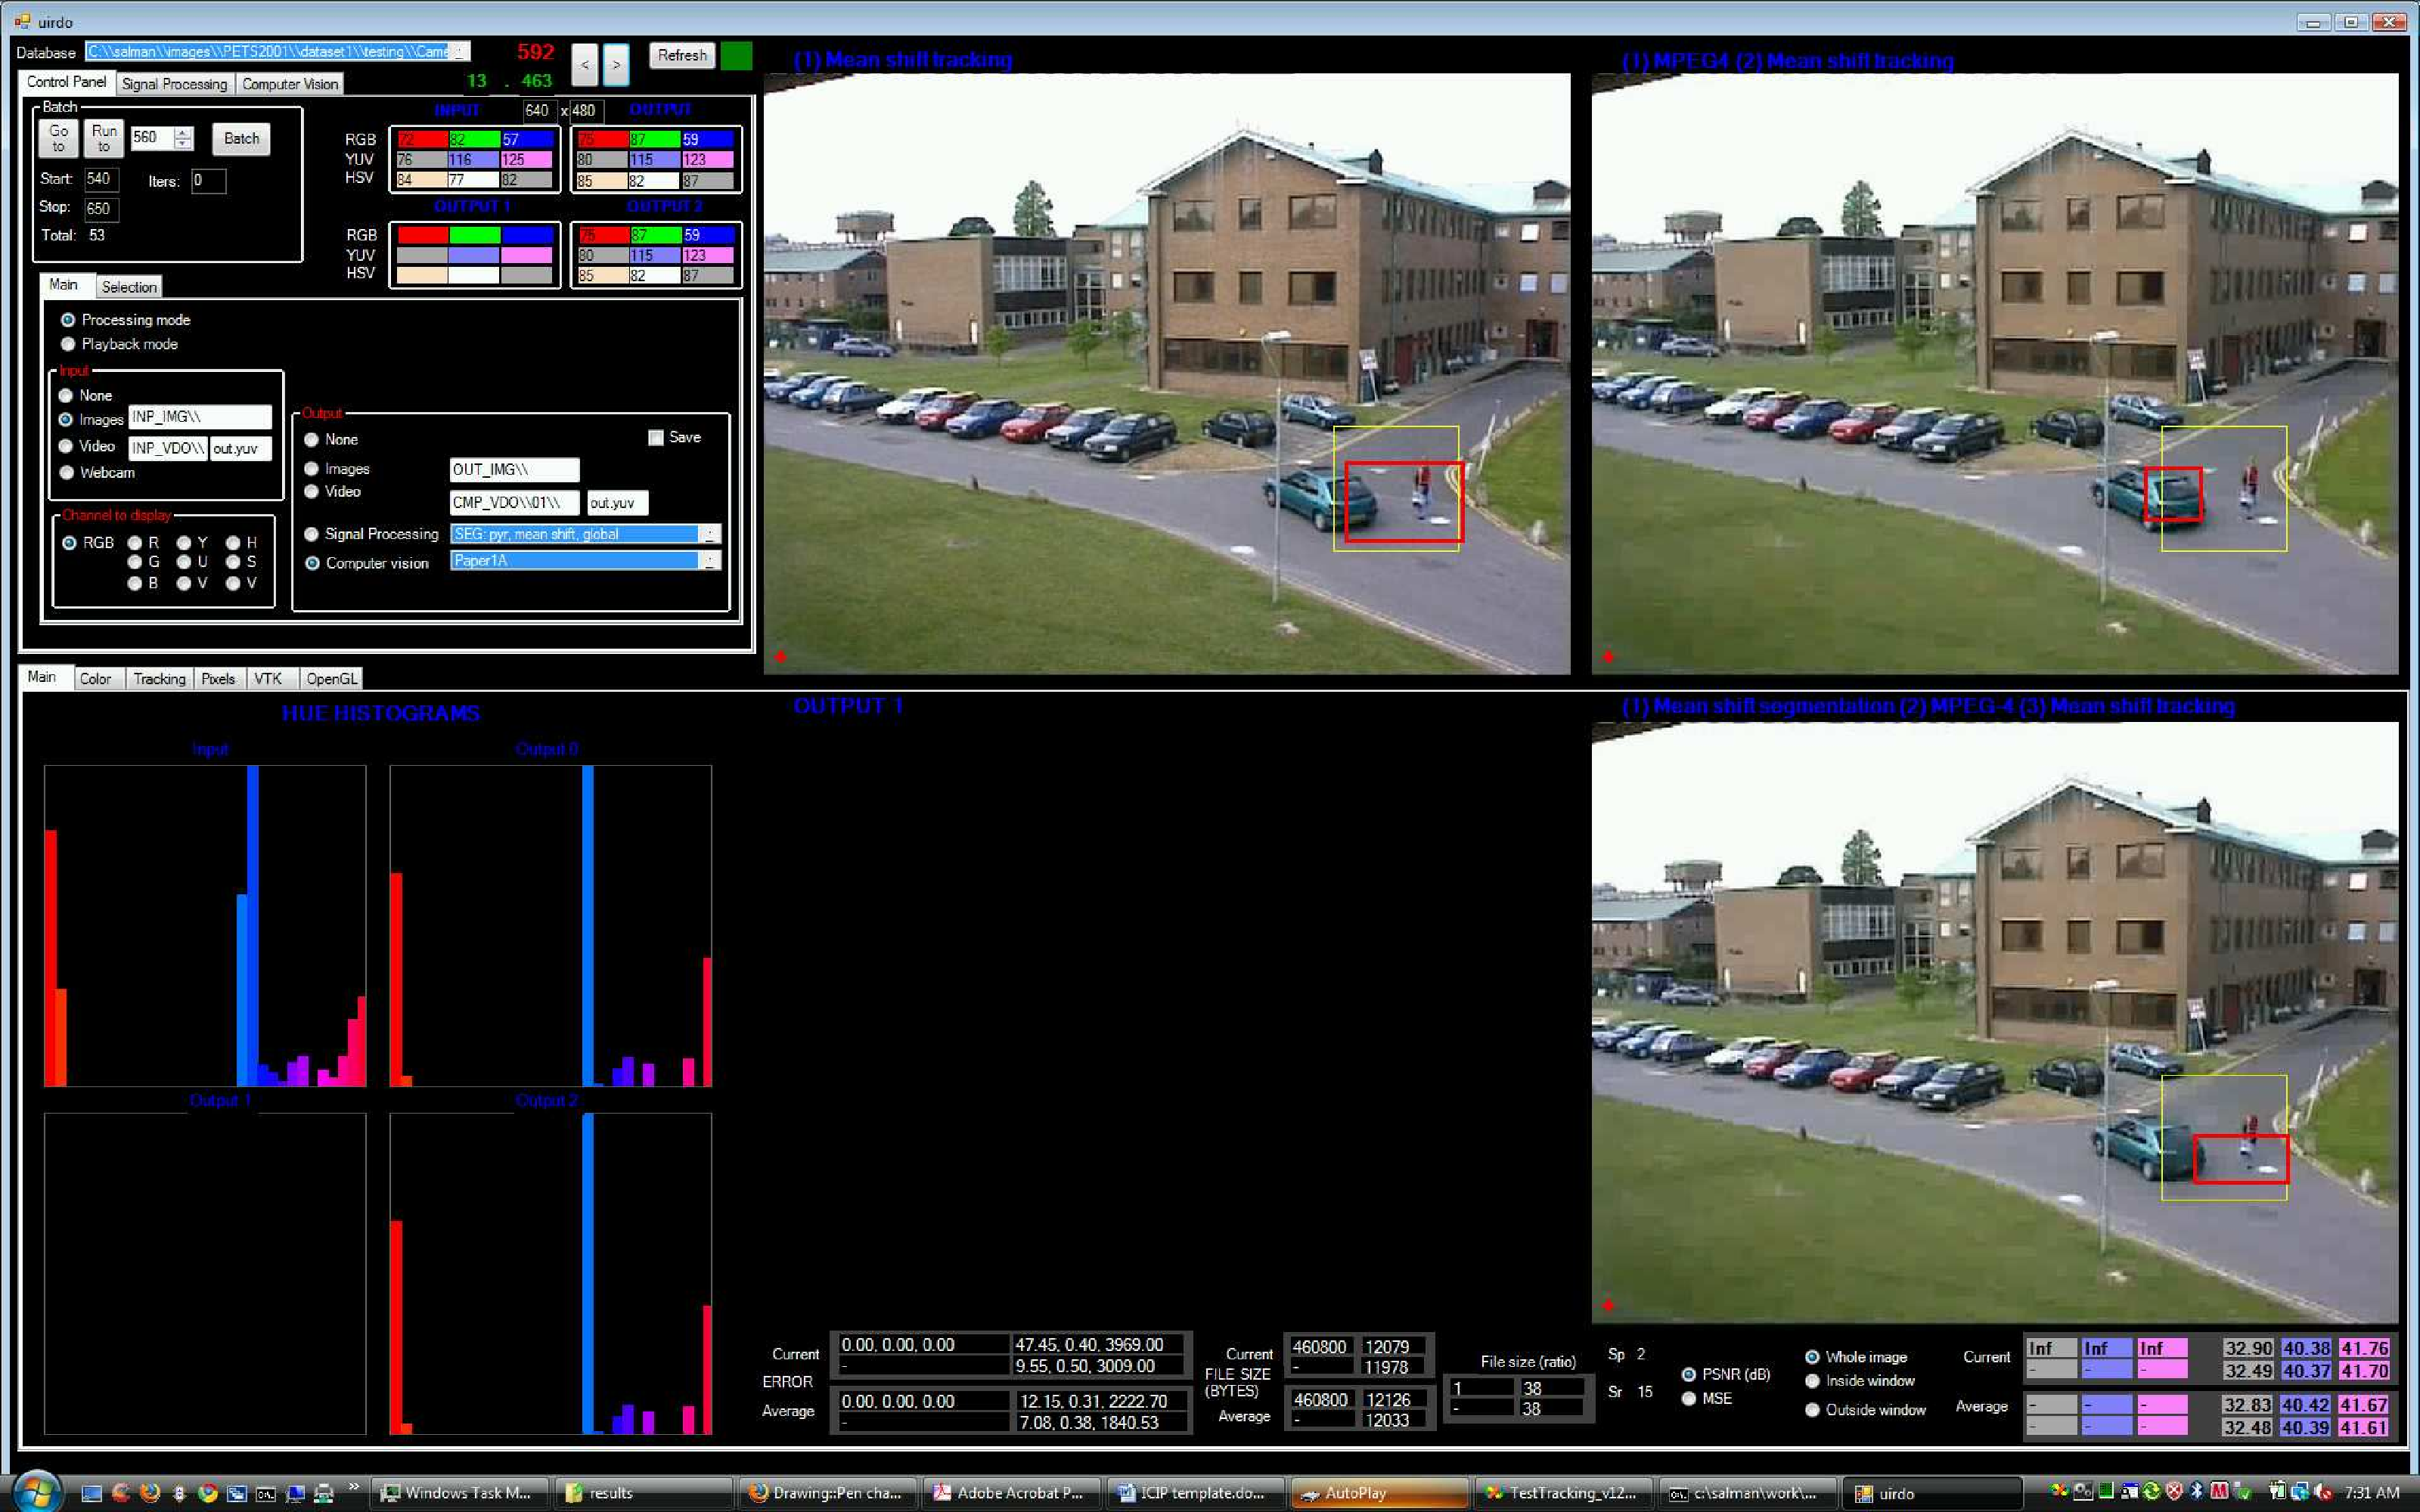
\includegraphics[width=.45\textwidth]{figs/ICIP2009_PETS2001_FN_00592_snapshotVVG}
			\caption{PETS2001  (a) Top left, Ground truth, (b) Top right, Tracker 1 looses track as the woman emerges from behind a car whose color distribution has some elements close to her own distribution.  (c) Bottom right, Tracker 2 holds track.  The target bounding box is shown in red.  The segmentation box is shown in yellow.  Note that it is shown for Tracker 1 only for illustration purposes, even though segmentation is not applied in this case.  In similar order, histograms of the target can be viewed in the bar graphs.}
\label{fig:PETS2001_Frame_592_small_size}
\end{figure}

%PETS2001: accuracy
\begin{figure}
			\centering

			\subfigure[Qp=5]
				{
					\includegraphics[width=.22\textwidth]{figs/ICIP2009_PETS2001_TrackingError_Qp_5}
					\label{fig:Accuracy_Qp_05_PETS2001}
				}
			\subfigure[Qp=16]
				{
					\includegraphics[width=.22\textwidth]{figs/ICIP2009_PETS2001_TrackingError_Qp_16}
					\label{fig:Accuracy_Qp_16_PETS2001}
				}
			\subfigure[Qp=27]
				{
					\includegraphics[width=.22\textwidth]{figs/ICIP2009_PETS2001_TrackingError_Qp_27}
					\label{fig:Accuracy_Qp_27_PETS2001}
				}
			\subfigure[Qp=31]
				{
					\includegraphics[width=.22\textwidth]{figs/ICIP2009_PETS2001_TrackingError_Qp_31}
					\label{fig:Accuracy_Qp_31_PETS2001}
				}
			\caption{PETS2001, tracking accuracy for different values of Qp.} 	
			\label{fig:Accuracy_PETS2001}	
			
\end{figure}

%PETS2001: bitrate
\begin{figure}
			\centering
			\includegraphics[width=.22\textwidth]{figs/ICIP2009_PETS2001_bitRateRatio}
			\caption{PETS2001, bitrate comparison.}
			\label{fig:Bitrate_comparison_PETS2001}			
\end{figure}

%PETS2001: PSNR
\begin{figure}
			\centering

			\subfigure[Whole image.]
				{
					\includegraphics[width=.22\textwidth]{figs/ICIP2009_PETS2001_PSNRdiffEntireImage}
					\label{fig:PSNR_whole_PETS2001}
				}
			\subfigure[Inside segmenation window.]
				{
					\includegraphics[width=.22\textwidth]{figs/ICIP2009_PETS2001_PSNRdiffROI}
					\label{fig:PSNR_window_PETS2001}
				}				
			\caption{PETS 2007, Luma PSNR.  Notice that there is more degradation in PSNR inside the segmented window.} 	
			\label{fig:PSNR_Comparison_PETS2001}	
\end{figure}

In step 3, the goal was to find a transformation that would, as explained in the introduction, help the computer vision algorithm run on the MPEG-4 output better than without the transformation.  The transformation that we picked is Mean Shift segmentation, which uses the same technique as the mean shift tracker to center its window on local histogram peaks.  At this stage, we made three decisions, (a) the class of the transformation to be used (b) the particular algorithm within that class (c) the parameters of the algorithm.  The class chosen was segmentation.  The particular algorithm within that class as stated above was Mean Shift segmentation.  As for the parameters, we iterate over the process of segmentation, compression, decompression, tracking, comparing results with the ground truth, and then choosing segmentation parameters that produce the best results.  All this is done automatically.  The reason for choosing mean shift segmentation was that since the mean shift tracker needs the backprojected window to compute its motion vectors, the mean shift segmentation may provide a better backprojection.  Even though that backprojection would undergo distortions through the MPEG-4 codec, it would still better preserve local hue information.  We did not segment the whole image, but only a window placed around the object of interest.  It was initialized in the same step as the mean shift tracker, and from there on, its position was updated automatically.  This setup is called Tracker 2 from here on.  

We compare Tracker 1 performance with the ground truth, and Tracker 2 performance with the ground truth.  In PETS2001, we track a person in a sparse background as she gets occluded by a car with a similar color distribution.  In PETS2007, we track a bag in a dense environment.  These two scenarios were chosen since they are quite different and would provide a better test of our approach.  Additionally, in both cases, the tracked object is occluded by another object with a similar color distribution.  This of course, presents one of the most significant challenges in tracking applications. 

%--------------------------------------------------------------------------------------------------------------------------------------------------------------
\section{RESULTS}
%--------------------------------------------------------------------------------------------------------------------------------------------------------------

We look at Trackers 1 and 2 from three angles: (a) performance, (b) quantity, in terms of bitrate (i.e. bandwidth used) and (c) quality, in terms of Euclidean distances of bounding boxes.  For PETS2001 and 2007, these are shown respectively in Figures~\ref{fig:Accuracy_PETS2001} and \ref{fig:Accuracy_PETS2007}, Figures~\ref{fig:Bitrate_comparison_PETS2001} and \ref{fig:Bitrate_comparison_PETS2007}, Figures~\ref{fig:PSNR_Comparison_PETS2001} and Figures \ref{fig:PSNR_Comparison_PETS2007}.  

Figures~\ref{fig:Accuracy_PETS2001} and \ref{fig:Accuracy_PETS2007} show that in all but one case, Tracker 2 produces better results than Tracker 1 at different values of the quantization parameter, $Qp$.  The tracking accuracy in these figures is measured in terms of Euclidean distances of bounding box centers.  Figures~\ref{fig:Bitrate_comparison_PETS2001} and \ref{fig:Bitrate_comparison_PETS2007} show a bitrate ratio between the trackers.  It is clear that Tracker 2 produces a slightly lower bitrate signal.  The reason is that the mean shift segmenter reduces some variability in the input signal.  Figures~\ref{fig:PSNR_Comparison_PETS2001} and Figures \ref{fig:PSNR_Comparison_PETS2007} display a comparison of luma PSNR of the overall image and inside the segmented window.  These figures present an interesting phenomenon.

First of all, it is obvious that there is a substantial tradeoff in luma PSNR inside the segmented window.  This is the price to pay if better tracking is required.  However, the price paid at lower bitrates, i.e. higher values of $Qp$ is less and less.  This is of course precisely when you would need a better tracker.  Now, our results show that tracking doesn't always get worse with higher values of $Qp$, but it's not entirely clear if this is always the case.  As of now, it presents an interesting insight that computer vision doesn't always get worse at lower bitrates.  This needs to be factored in when finding the transformation $g(x,y)$.

Also, as shown in Figure~\ref{fig:Accuracy_Qp_31_PETS2007}, this is the only scenario where Tracker 2 performs significantly lower than Tracker 1.  The reason is that the bag being tracked is occluded by a person with a similar color distribution.  At some values of $Qp$, part of the object being tracked and part of the occluding object which end up in the same macroblock, may be coded uniformly throwing the tracker of course.  This presents a fundamental challenge in block based codecs since the block boundaries are not aligned with the computer vision algorithm boundaries.

%PETS2007: picture	
\begin{figure}
			\centering
			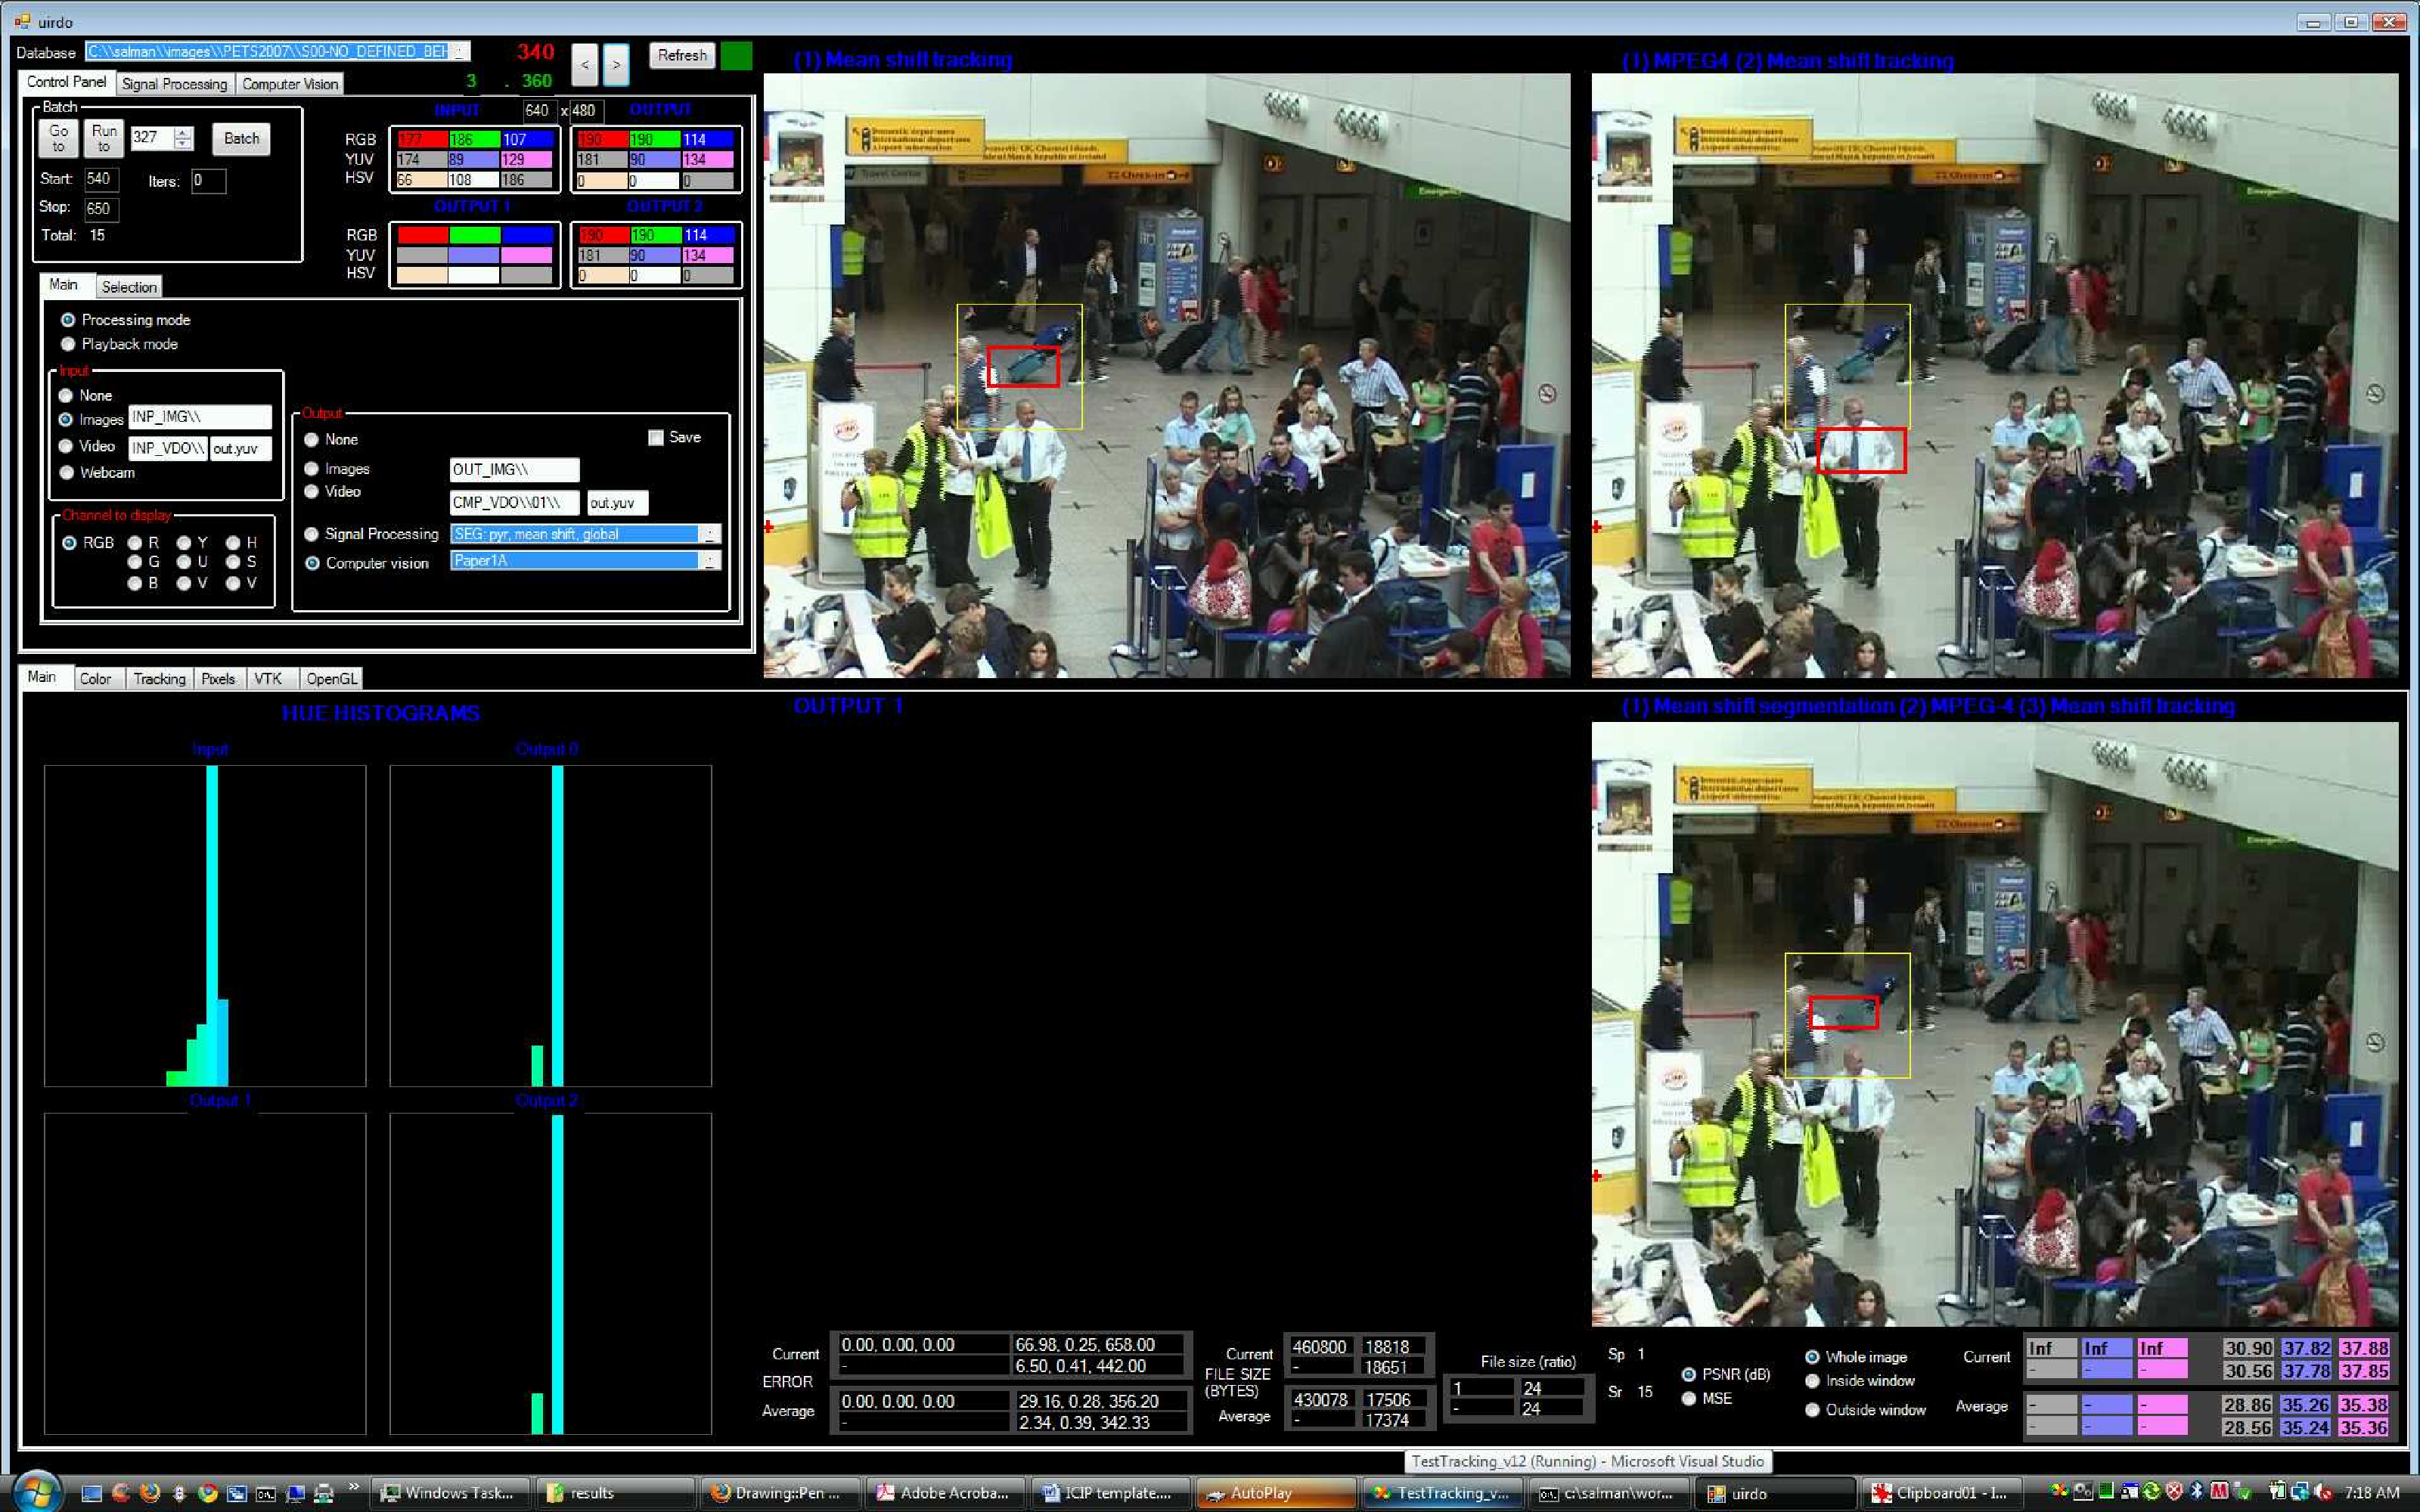
\includegraphics[width=.45\textwidth]{figs/ICIP2009_PETS2007_FN_00340_snapshotVVG}
			\caption{PETS2007.}
			\label{fig:ExperimentalSetup2}
\end{figure}

%PETS2007: accuracy
\begin{figure}
			\centering

			\subfigure[Qp=5]
				{
					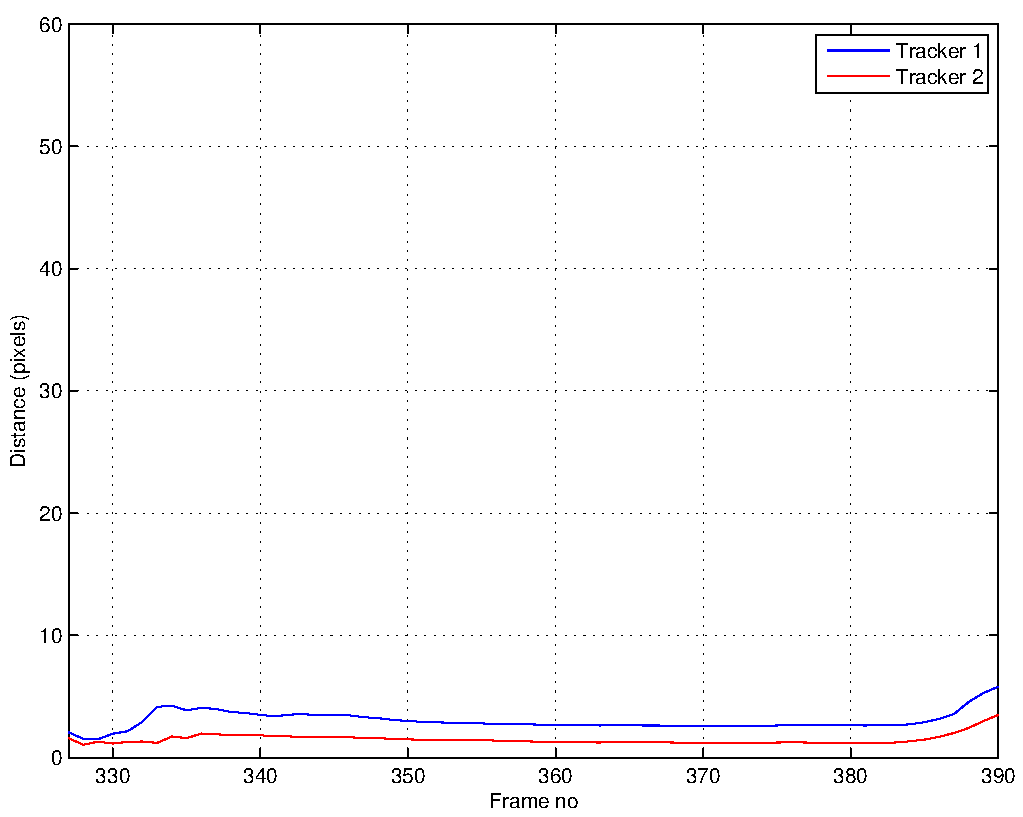
\includegraphics[width=.22\textwidth]{figs/ICIP2009_PETS2007_TrackingError_Qp_5}
					\label{fig:Accuracy_Qp_05_PETS2007}
				}
			\subfigure[Qp=16]
				{
					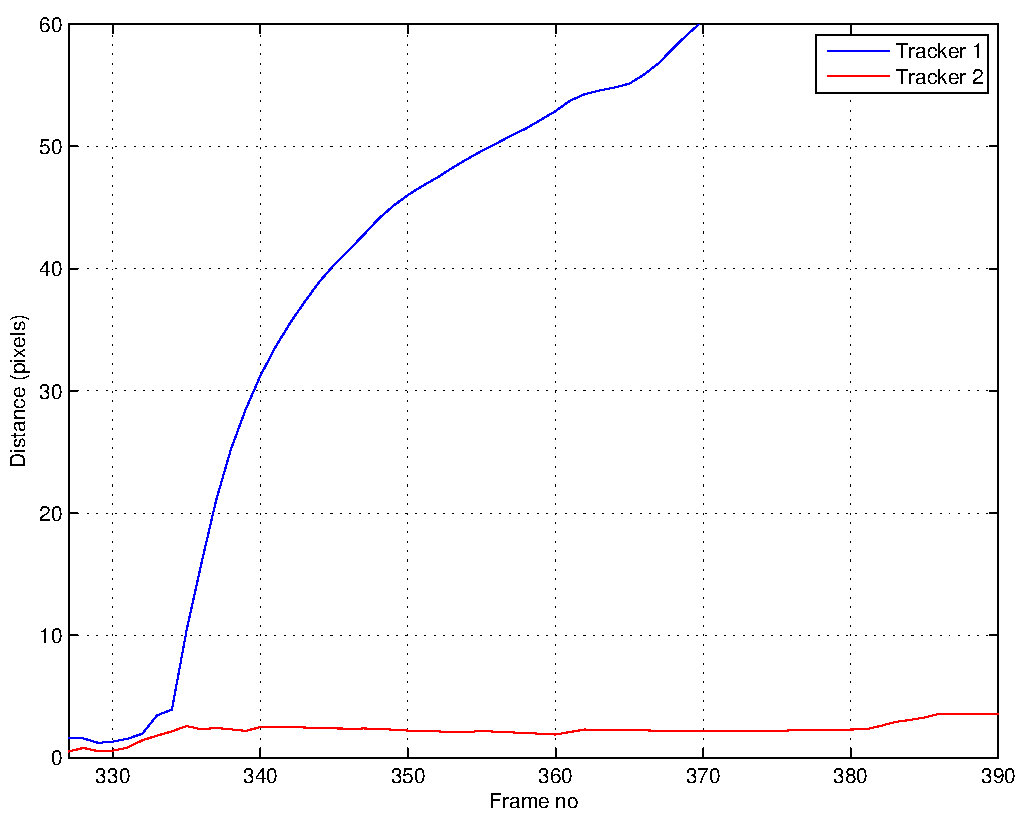
\includegraphics[width=.22\textwidth]{figs/ICIP2009_PETS2007_TrackingError_Qp_16}
					\label{fig:Accuracy_Qp_16_PETS2007}
				}
			\subfigure[Qp=27]
				{
					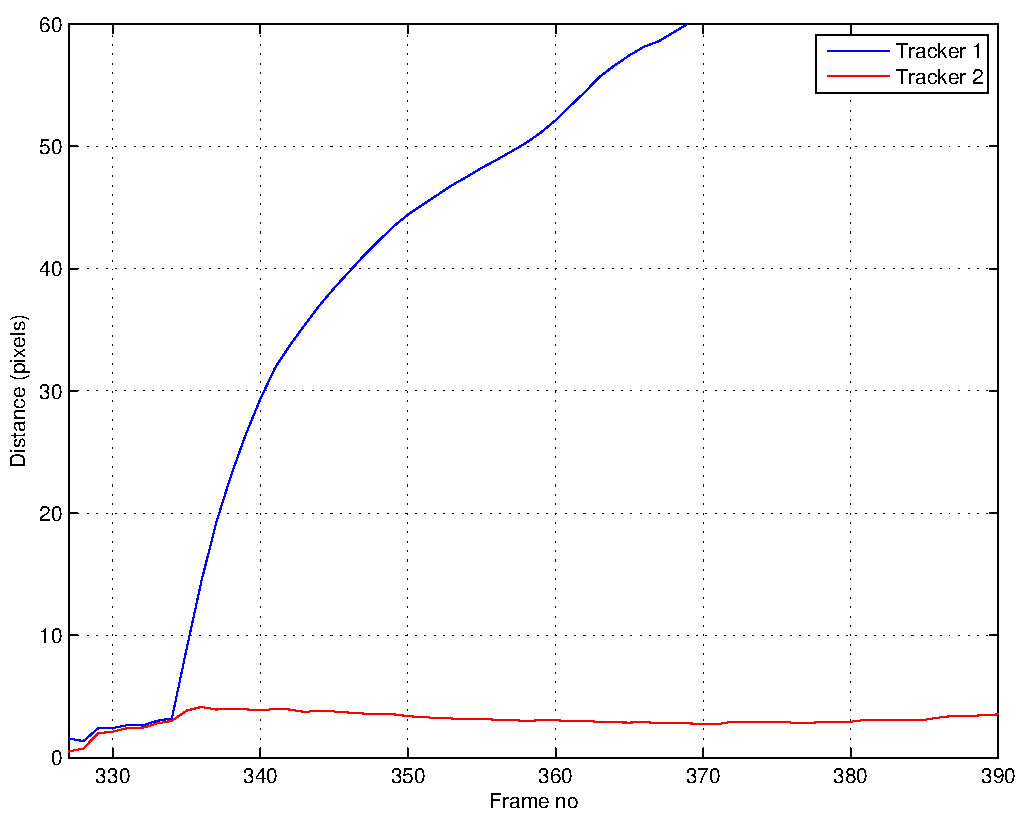
\includegraphics[width=.22\textwidth]{figs/ICIP2009_PETS2007_TrackingError_Qp_27}
					\label{fig:Accuracy_Qp_27_PETS2007}
				}
			\subfigure[Qp=31]
				{
					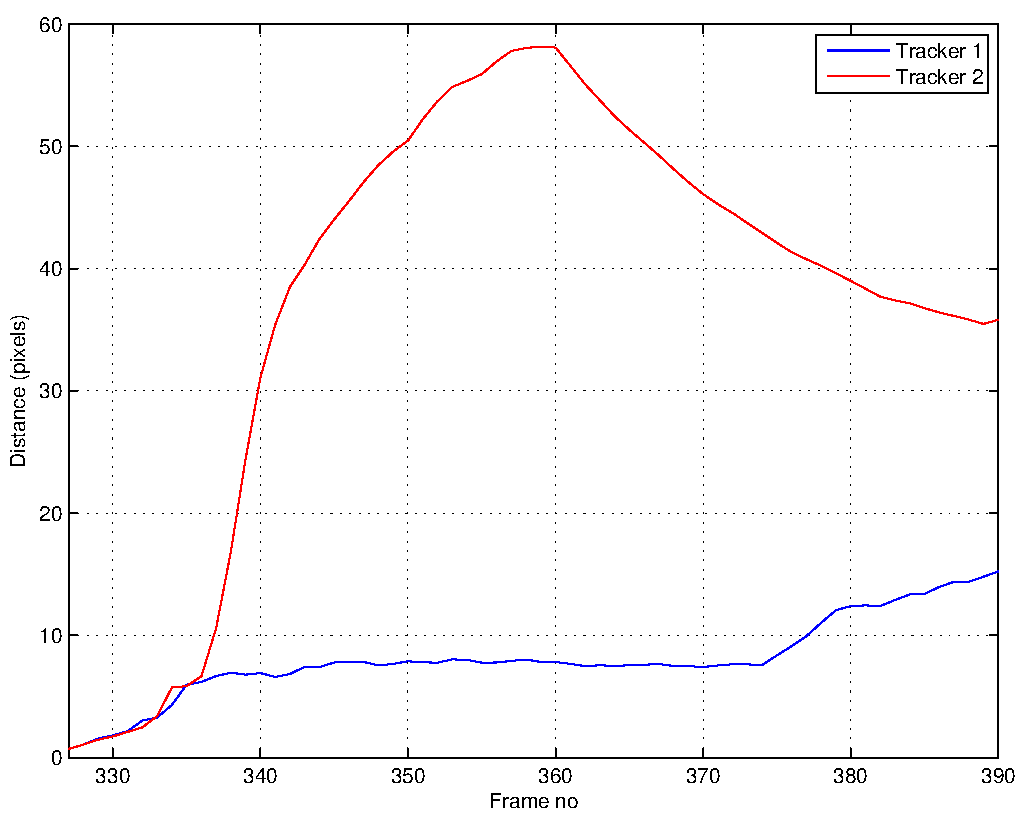
\includegraphics[width=.22\textwidth]{figs/ICIP2009_PETS2007_TrackingError_Qp_31}
					\label{fig:Accuracy_Qp_31_PETS2007}
				}
				
			\caption{PETS2007, tracking accuracy for different values of Qp.} 	
			\label{fig:Accuracy_PETS2007}	
\end{figure}

%PETS2007: bitrate
\begin{figure}
			\centering
			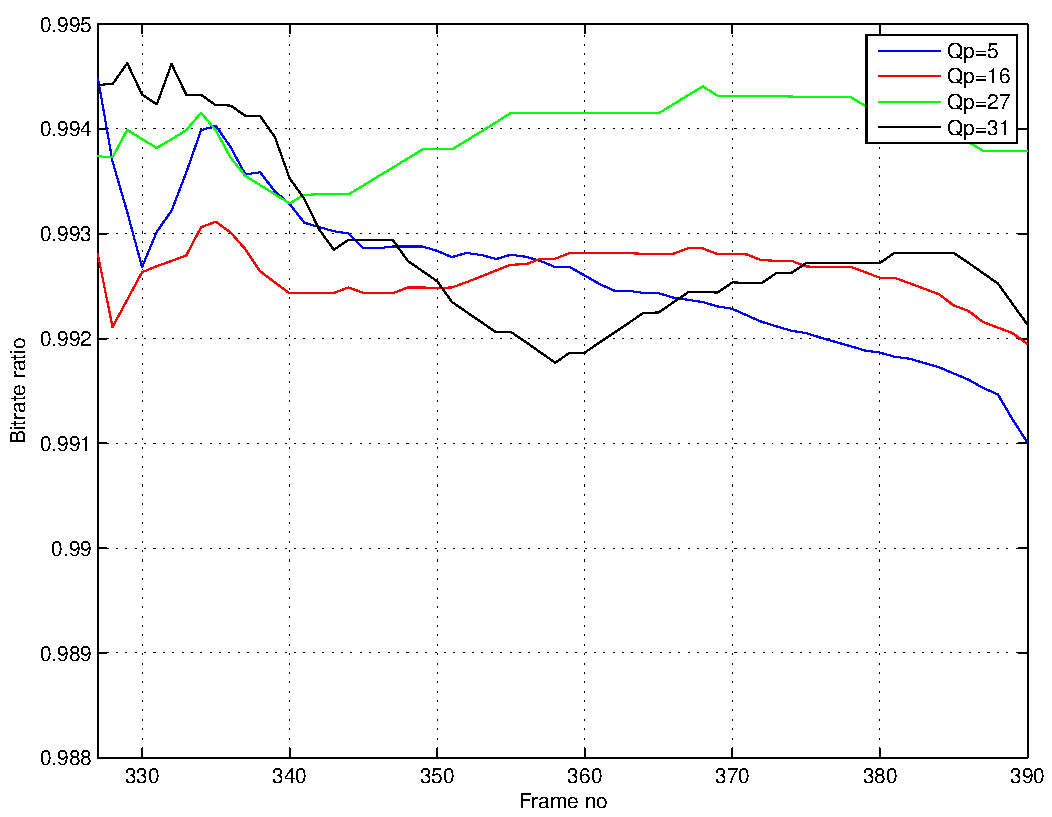
\includegraphics[width=.22\textwidth]{figs/ICIP2009_PETS2007_bitRateRatio}
			\caption{PETS2007, bitrate comparison.}
			\label{fig:Bitrate_comparison_PETS2007}
			 					
\end{figure}

%PETS2007: PSNR
\begin{figure}
			\centering

			\subfigure[Whole image.]
				{
					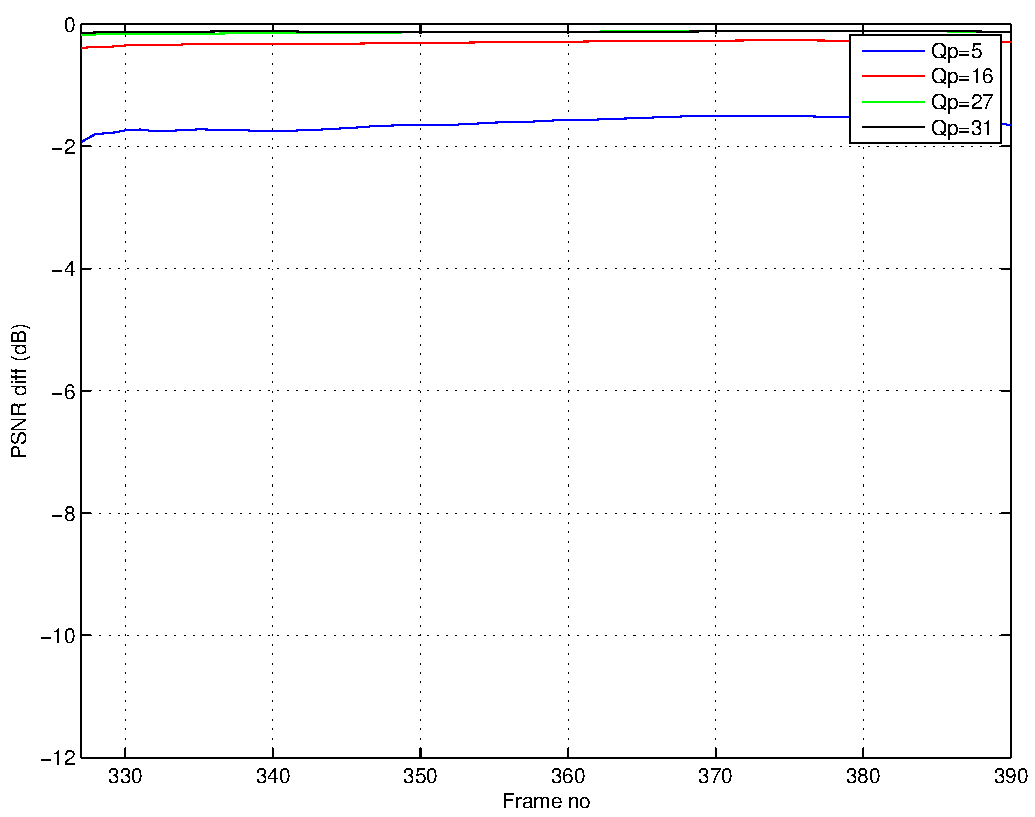
\includegraphics[width=.22\textwidth]{figs/ICIP2009_PETS2007_PSNRdiffEntireImage}
					\label{fig:PSNR_whole_PETS2007}
				}
			\subfigure[Inside segmentation window.]
				{
					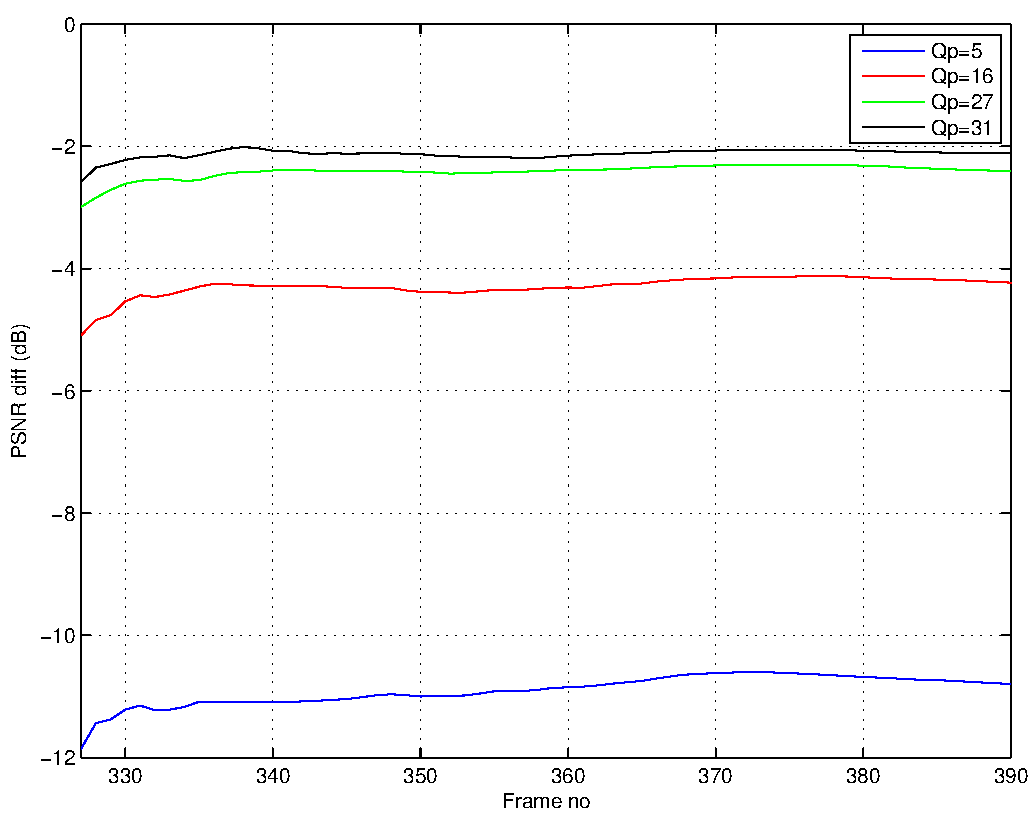
\includegraphics[width=.22\textwidth]{figs/ICIP2009_PETS2007_PSNRdiffROI}
					\label{fig:PSNR_window_PETS2007}
				}				
			\caption{PETS 2007, Luma PSNR.  Notice that there is more degradation in PSNR inside the segmented window.} 	
			\label{fig:PSNR_Comparison_PETS2007}	
\end{figure}

%--------------------------------------------------------------------------------------------------------------------------------------------------------------
\section{CONCLUSIONS}
%--------------------------------------------------------------------------------------------------------------------------------------------------------------
Our broad goal was to understand how to preserve information in an input image so that it would run a given computer vision algorithm better on the output of a codec.  For this purpose, we picked a specific computer vision algorithm, mean shift tracking, applied a transformation to it, mean shift segmentation, iterated over its parameters, and saw that in most cases, performance is improved over the scenario when the same computer vision algorithm is applied to an untransformed image.  We saw that this comes at a cost of lower PSNR.  It now depends on the application at hand if that cost is justifiable.  We on our part, will continue to study the tradeoffs involved in such scenarios, using a broader class of computer vision algorithms, a broader class of codecs, and of course, a broader class of image transformations.


\bibliographystyle{ieee}
\bibliography{c:/salman/work/writing/MyCitations}

\end{document}
